\documentclass[]{article}   % list options between brackets
\setlength{\parskip}{\baselineskip}%
\setlength{\parindent}{0pt}%
\usepackage{enumitem}
\usepackage{hyperref}              % list packages between braces
\usepackage{amsfonts}
\usepackage{amsmath}
% to use includegraphics
\usepackage{graphicx}

% type user-defined commands here

\begin{document}

\title{CS2361: Blockchain and Cryptocurrencies\\ Project Report: M-Pin}   % type title between braces
\author{Argha Chakrabarty \and Aarav Varshney}         % type author(s) between braces
\date{May 1, 2022}    % type date between braces
\maketitle

\section*{Introduction}
We need authentication for primarily three reasons:
\begin{itemize}
    \itemsep0em
    \item authenticate the client to the server,
    \item authenticate the server to the client,
    \item and should result in a negotiated encryption key with which subsequent communications can be encrypted.
\end{itemize}
Until now we've been using Username/Password authentication for authenticating the client and the use of SSL/TLS protocols for authenticating the server. SSL even though now deprecated still had some good ideas but the Username/Password is extremely vulnerable to exploits and that's why there is a massive shift to Multi Factor Authentication (MFA).

The biggest exploit for username/password authentication is that the server stores either the hash of the password or the password itself in the database which if compromised can be used to gain access to the passwords.

The idea behind M-Pin is that each registered client is issued with a large cryptographic secret. They then prove to the server that they are in possession of this secret using a zero-knowledge proof. This removes the requirement for any information related to client secrets to be stored on the server.

Another crucial attribute of M-Pin is the use of third party authentication. Similar to how SSL uses a CA to verify the certificates, M-Pin uses Trusted Authority (TA) to store the secrets in contrast to Username/Password where the server performs regular operations as well as authentication.

\newpage
\section*{Technical Details}
\subsection*{Concepts Utilized}
\begin{itemize}
    \item Pairing Based Cryptography: It is based on pairing functions that map pairs of points on an elliptic curve into a finite field.
    \item Identity Based Encryption: When communicating with someone using their public key, there is always a concern whether the public key belongs to intended party or some adversary. We see the usage of CAs to verify the legitimacy of the public key in PKIs. IBE proposed that the public key should be composed of some identifying information such as email address.
    \item  Replay Attack: The attacker can capture the encrypted message sent to a trusted party and send it again at a later time. For instance, if an attacker captures a request for a financial txn, they can send the request again to make another txn.
\end{itemize}
\subsection*{Working of M-Pin}
\subsubsection*{Notations}
\begin{itemize}
    \item $ID_a$: The client's email address.
    \item q denotes the size of the field over which our elliptic curve E is defined.
    \item $G_1$ is a subgroup of $E(F_q )$, $G_2$ is a subgroup of $E(F_{q^k} )$, where k is a parameter  called the embedding degree.
    \item $H_1$ a hash function which maps to a point on $G_1$
    \item $H_2$ a hash function which maps to a point on $G_2$
    \item $e: G_1 \times  G_2 \rightarrow $$\mathbb{Z}_q$
    \item s $\in$ $\mathbb{Z}_q$: The master secret stored with the TA.
    \item sA: The client's secret key.
    \item 'x' a random number in $Z_q$
    \item 'y' a random number in $Z_q$
\end{itemize}
\newpage
\subsubsection*{Step 1: Key Generation}
The client computes point A on the eclipse curve using a $ID_a$ which is then sent to the TA to get client secret key sA where s is a master secret stored in the TA.
\paragraph*{Process}
\begin{enumerate}
    \item Client: $A \leftarrow H_1(ID_a) $
    \item TA: Calculates $sA$
    \item Client: The client calculates the token $((s-\alpha)A)$ using his own PIN $(\alpha)$ and stores the token in local storage.
\end{enumerate}
\subsubsection*{Step 2: Authentication}
Communication between the client and the server takes place.
\paragraph*{Process}
\begin{enumerate}
    \item Client: Receives pin $\alpha$ from the user, picks x.
    \item Client: Computes $U \leftarrow xA$.
    \item Client: Sends \{$ID_a, U$\} to the server.
    \item Server: Sends y to the client.
    \item Client: Computes $V \leftarrow -(x+y)((s-\alpha)A +\alpha A)$ and sends V to the server.
    \item Server: Computes $D \leftarrow H_1(ID_a)$ and \newline $g \leftarrow e(V,Q)e(U+yD,sQ)$.
    \item If $g = 1$ then the client is authenticated.
\end{enumerate}
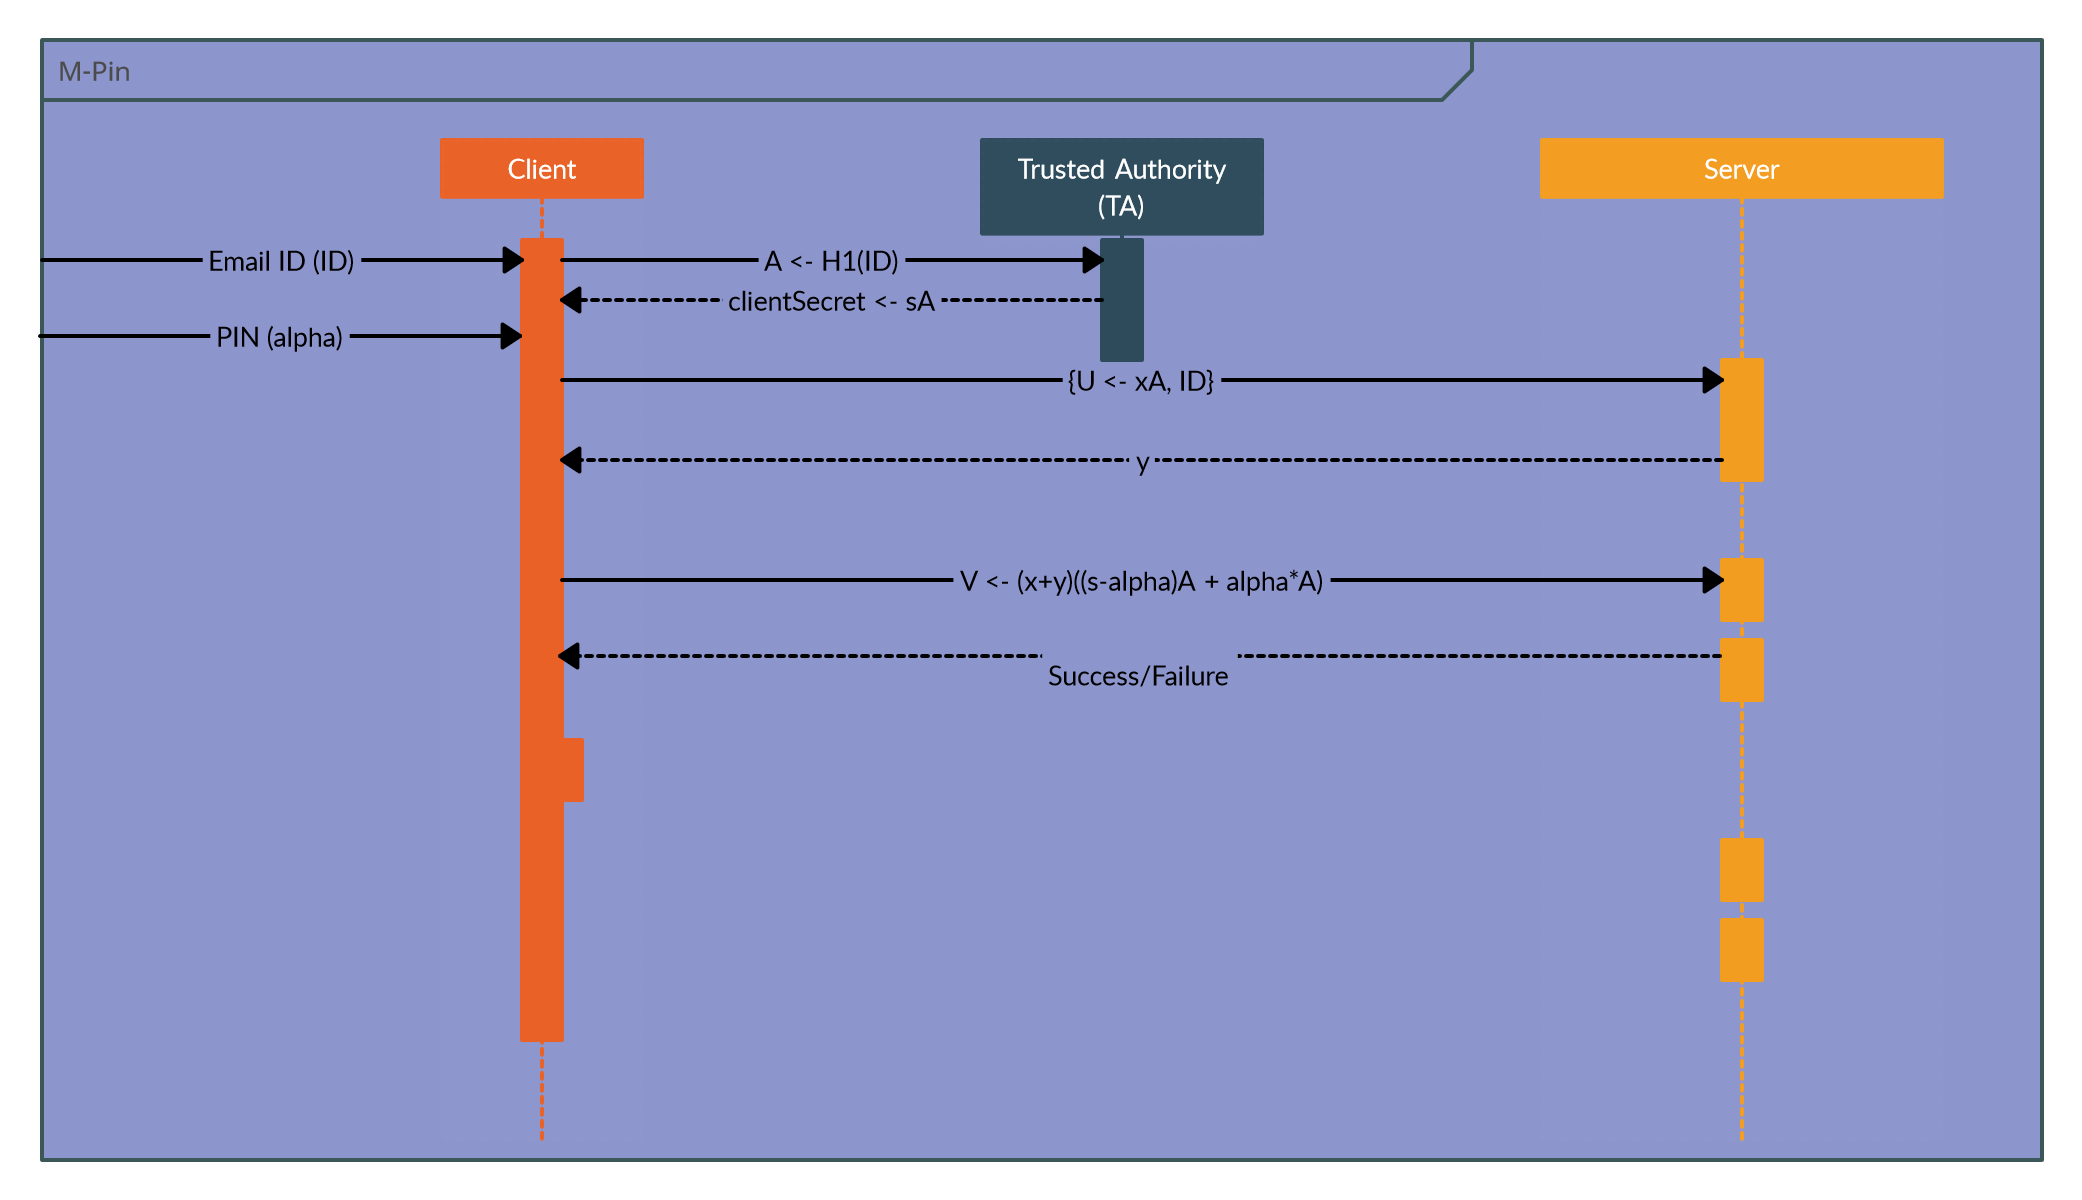
\includegraphics[width=\textwidth]{./mpin-process.png}
\newpage
\section*{Analysis}
\subsection*{Security}
\begin{itemize}
    \item The server does not store user's hashed password or any detail that may compromise their identity on the platform. 
    \item There are two points of failure. An adversary even if acquire user's pin they would still require the token to generate the client secret. 
    \item There is no efficiently computable $\psi$:G2$\rightarrow$G1 in Type 3 Pairing. \cite{Steven:2013}
    \item The type-3 pairing allows us to assume Symmentric External \\ Diffie-Helman (SXDH) assumption which futher imposes a set of assumption:
    \begin{itemize}
        \item The discrete logarithm problem (DLP), the computational Diffie-Hellman problem (CDH), and the computational co-Diffie-Hellman problem are all intractable in ${\displaystyle {\mathbb {G} }_{1}}$ and$ {\displaystyle {\mathbb {G} }_{2}} $
        \item There exists an efficiently computable bilinear map  \\(pairing) ${\displaystyle e(\cdot ,\cdot ):{\mathbb {G} }_{1}\times {\mathbb {G} }_{2}\rightarrow {\mathbb {G} }_{T}} $
        \item The decisional Diffie-Hellman problem (DDH) is intractable in
        ${\displaystyle {\mathbb {G} }_{1}}$ and ${\mathbb {G} }_{2}.$
    \end{itemize}

    \item er (aP, bQ) = er $(P, Q)^ab$ for all a, b $\in$ Fr (Bilinearity)
    \item We use BN-254 Elliptic Curve to implement M-Pin. The curve has an embedding degree of 12 and is know to be secure and calculating pairing is efficient and is used by Aztec for Ethereum. \cite{Aztec:2013}

\subsection*{Verification}
The server can verify the authenticity of the client by calculating $$g=e(V, Q).e(U + yA, sQ)$$. If $g=1$ then the client is authenticated.
\begin{align*}
    g &= e(V, Q)e(U + yA, sQ) \\
    &= e(-(x+y)((s-\alpha)A +\alpha A), sQ).e(U + yA, sQ) \\
    &= e(-(x+y)(sA), Q).e(xA + yA, sQ) \\
    &= e(-(x+y)(A), sQ).e((x + y)A, sQ) \\
    &= e((x+y)(A), sQ)^{-1}.e((x+y)A, sQ) \\
    &= 1
\end{align*}


\end{itemize}

\section*{Plan for the Project}
Our major inspiration for implementation of the project comes from the implementation by \href{https://web.archive.org/web/20161107110119/http://docs.milagro.io/en/mfa/getting-started/milagro-mfa-developer-guide.html}{Apache's Milagro MFA} which although is now deprecated but has clear implementation ideas.

Beforehand, the groups $G_1, G_2$ and $G_T$ are fixed. Along with $G_1, G_2$ and $G_T$, their corresponding hashing functions are also generated which maps any data to a point on the curve. For example $H_1$ will map the email id of Alice to $G_1$. $H1(alice@bob.com) = A$.

\begin{enumerate}
    \item Client Side:
        \begin{enumerate}
            \item We have created the client side for the app in React.js.
            \item The client handles the input of the pin and the id (email) after which communication takes place between the TA to compute client secret. We primarily use \href{https://www.npmjs.com/package/crypto-js}{ crypto-js } for the computation of the tokens and keys.
        \end{enumerate}
    \item Server Side:
    \begin{enumerate}
        \item Due to ease of availabilty of crypto libraries and elliptic curve libraries, we are using Python to build our server.
        \item The server also communicates with a small mongo database to store client ids, nonce which are deleted after expiry. 
        \item We store the server secret in server. The server returns a response with a success or failure message based on the result of authentication. 
    \end{enumerate}
    \item TA:
    \begin{enumerate}
        \item The TA will generate a master secret for each of it's servers $s$, and will issue a server secret $S = sQ$.

        \item When a client, Alice reaches out to the TA for the initial authentication, she will be assigned a client secret, $D = sA$, where A is Alice's email-id or any identification unique to Alice hashed to a point in $G_1$.
    \end{enumerate}
\end{enumerate}
\newpage
\section*{Future Ideas / Plans for expansions}
\begin{enumerate}
    \item To implement mutiple TAs (DTA) to safegaurd against a single  point of failure. This is possible due to pairing based cryptography.
    \item Also, to implement a scoring based for multiple wrong attempts at authentication to prevent brute force attacks while also making the system more user friendly as suggested in the paper [3]. 
    \item The entire process suffers from one flaw which is that it takes three passes between the client and the server which if the server also carries out username/password based authentication will find it difficult to change protocol. The paper titled "Milagro Multi-Factor Authentication" proposes e-M-Pin that uses a single pass between the client and the server.

    The one pass authentication poses the problem of Replay Attack which is why we now also use current time: a) CCT: Current Client Time, b) SCT: Current Server Time and a single use arbitary number, nonce.
    
    The new process is only slightly different:
    \begin{enumerate}
        \item The client now also generates a nonce in $Z_q$ along with x and stores the current time.
        \item y is now computed as: $y \leftarrow H_q (ID_a || U || W || nonce || CCT).$
        \item and the client sends: {IDa,U,W,V,nonce,CCT} to the server.
        \item The server first checks if the SCT - CCT falls within the expiration time (t) else fail the authentication. Secondly, verify if the nonce has been used already or not.
        \item Finally, save the nonce and calculate y as \newline $y \leftarrow H_q (ID_a || U || W || nonce || CCT).$
    \end{enumerate}
    
\end{enumerate}

\section*{Links}
\subsection*{Backend}
Github: \url{https://github.com/aarav22/mpin-backend} \\
Hosted: \url{3.108.58.123}
\subsection*{Frontend}
Github: \url{https://github.com/argha-dot/mPins-frontend} \\
Hosted: \url{3.110.108.83:5000}
\subsection*{Video}
\url{https://www.youtube.com/watch?v=Q_X_Q_X_Q_X}


\nocite{*}
\bibliographystyle{plain}
\bibliography{ref}

\end{document}
